% The LaTeX template for the master's thesis 
% Degree Program: Computational Engineering and Technical Physics (LATE)
% University: LUT University, Finland
% Date: April 7, 2022

% Tested to work in overleaf.

% The instructions about the abstract in Finnish:
% 1) Students who have not received their basic education in Finnish or Swedish 
% always write their abstract only in English.
% 2) Students whose language of their basic education is Finnish or Swedish:  
% always write the abstract also in Finnish or Swedish, depending on the language of their basic education. 


% The template for the Finnish abstract added.

\documentclass{lutmscthesis}[2017/10/03]

\usepackage[utf8]{inputenc}
\usepackage[T1]{fontenc}
\usepackage[english]{babel}

\usepackage{times}
\usepackage{tabularx}
\usepackage{multirow}

\usepackage{setspace}
\usepackage{verbatim}
\usepackage[intlimits]{amsmath}
\usepackage{enumitem}

% The abbreviations
\usepackage[acronym,nomain,nonumberlist]{glossaries}
\makeglossaries
\newacronym{2d}{2-D}{two-dimensional}
\newacronym{nhl}{NHL}{National Hockey League}
\newacronym{ppv}{PPV}{Positive Predictive Value}
\newacronym{tp}{TP}{True Positive}
\newacronym{fp}{FP}{False Positive}

\usepackage{pgfplots} 
\pgfplotsset{compat=newest} 
\newlength\figurewidth
\newlength\figureheight

\usepackage{float}
\floatstyle{plain}\restylefloat{figure}
\floatstyle{plaintop}\restylefloat{table}

\usepackage[pdfborder={0 0 0}]{hyperref}
\usepackage[]{algorithm}
\usepackage{cite}

\usepackage[figure,table]{totalcount}

\graphicspath{{resources/}}

\newcommand{\vect}[1]{\boldsymbol{#1}}
\newcommand{\matr}[1]{\boldsymbol{#1}}
\newcommand{\diag}[1]{\mathrm{diag}(#1)}
\newcommand{\iprod}[1]{\left\langle #1 \right\rangle}
\newcommand{\me}{\mathrm{e}}
\newcommand{\mi}{\mathrm{i}}
\newcommand{\md}{\mathrm{d}}
\newcommand{\sse}{{}} %\mathrm{SSE}}
\newcommand{\trace}{\mathrm{Tr}\:}
\newcommand{\frp}[2]{{}^\mathrm{#1}\vect{#2}}
\newcommand{\frs}[3]{{}^\mathrm{#1}#2_\mathrm{#3}}
\newcommand{\frv}[3]{{}^\mathrm{#1}\vect{#2}_\mathrm{#3}}
\newcommand{\frm}[3]{{}^\mathrm{#1}\matr{#2}_\mathrm{#3}}
\newcommand{\colvec}[2]{\genfrac{[}{]}{0pt}{1}{#1}{#2}}
\newcommand{\relphantom}[1]{\mathrel{\phantom{#1}}}
\newcommand\aug{\fboxsep=-\fboxrule\!\!\!\fbox{\strut}\!\!\!}

\newcommand{\etal}{\textit{et al}. }

\newtheorem{theorem}{Theorem}

% Thesis information

\author{Arno Törö, 0570180}

\title{A Case Study on Flappy Bird AI}

\Keywords{hakusana1, hakusana2}

% The official examiners of your thesis
\FirstExaminer{Professori Heikki K\"alvi\"ainen}

\Year{December 10, 2024}

% Thesis statistics for the abstract: number of pages, figures, tables, and appendices.

\addtostats{x sivua, y kuvaa, z taulukkoa, w liitettä}


\begin{document}
\selectlanguage{english}

\maketitle

\newpage

% \begin{abstract}

% Tiivistelmällä opiskelija osoittaa perehtyneisyyttä opinnäytteensä alaan ja aiheeseen ja se on objektiivinen, itsenäinen esitys opinnäytteestä. Tiivistelmän tulee olla ymmärrettävissä sellaisenaan ilman alkuperäisdokumenttia. Tiivistelmässä esitetään työn tavoite, menetelmät, tulokset ja johtopäätökset. Tiivistelmä on huolellisesti kirjoitettua tekstiä, jolla osoitetaan koulusivistyskielen hallinta. Tiivistelmän pituus on yksi A4-sivu. Tiivistelmä muotoillaan yhden rivivälillä.

% Kandidaatintyön tiivistelmä toimii kandidaatin tutkinnon kypsyysnäytteenä. Koulutusohjelmilla voi olla myös omia ohjeistuksia tiivistelmän kirjoittamisesta. Jos kandidaatintyö on tehty parityönä, kumpikin opiskelija kirjoittaa työstä oman tiivistelmänsä, joka toimii opiskelijan kypsyysnäytteenä. Kun tiivistelmä toimitetaan arvioitavaksi kypsyysnäytteenä, siinä täytyy myös olla kirjoittajan opiskelijanumero.

% \end{abstract}

% \selectlanguage{english}



% % These name-definitions must be after Babel language change
% % commands, as they redefine these.

% \renewcommand\refname{LÄHTEET}
% \renewcommand\contentsname{SISÄLLYSLUETTELO}

% \pagestyle{masters}



% % ---------------------------------------
% %    LIST OF SYMBOLS AND ABBREVIATIONS
% % ---------------------------------------

% \glsnogroupskiptrue
% \setlength{\glsdescwidth}{1.0\hsize}
% \printglossary[title=LIST OF ABBREVIATIONS,type=\acronymtype, style=long, nonumberlist, nopostdot]

% % Advice: All symbols and abbreviations are listed on this page in the alphabetical order. 
% % Remember to introduce the abbreviation when it is used in the text for the first time.\\

% % You may use the automated system, depending on your LaTeX environment:
% % \begin{verbatim}
% % \glsnogroupskiptrue
% % \setlength{\glsdescwidth}{1.0\hsize}
% % \printglossary[title=LIST OF ABBREVIATIONS,type=\acronymtype, 
% % style=long, nonumberlist, nopostdot]
% % \end{verbatim}

% % Adding manually
% \section*{SYMBOLI- JA LYHENNELUETTELO}

% \begin{tabular}{l l}
% 2-D & two-dimensional\\
% NHL & National Hockey League\\
% \vdots&\\
% \end{tabular}\\


% \newpage


% % ---------------------------------------
% %           TABLE OF CONTENTS
% % ---------------------------------------

% \tableofcontents


% % space between paragraphs
% \setlength{\parskip}{3ex}


% % ---------------------------------------
% %             INTRODUCTION
% % ---------------------------------------
\section{INTRODUCTION}
The game "Flappy Bird" was released in May 2013 and gained viral popularity in early 2014. The game gained popularity with its simple and minimalist gameplay mechanics, which were both addictive and frustrating for many players. In Flappy Bird, the players must navigate a bird between vertically moving pipes. The player earns one point for each pipe successfully passed.\\

This case study focuses on developing an AI agent to play Flappy Bird and beat a score of 100 in the game, which is considered challenging by the players. \cite{flappy_score} 


% Introduction: background, motivation and justification for the selected agent.

% Flappy Bird is a simple yet challenging arcade game in which the player controls a bird that must navigate between moving pipes. Despite the game looking easy, the game's non-intuitive controls make it a tough task for humans and an interesting challenge for AI.

% Motivation and Challenges:
% \begin{itemize}
%     \item Develop an understanding of reinforcement learning algorithms through a fun and interactive project.
%     \item A perfect use case for RL, requiring the agent to learn precise control over the bird's movement while adapting to moving level layouts in real time.
%     \item Building a Flappy Bird environment where a reinforcement learning model can continuously improve through trial and error.
% \end{itemize}
%Of course we could elaborate more, but why talk when a picture is all you need.


% \begin{figure}[ht]
%     \fbox{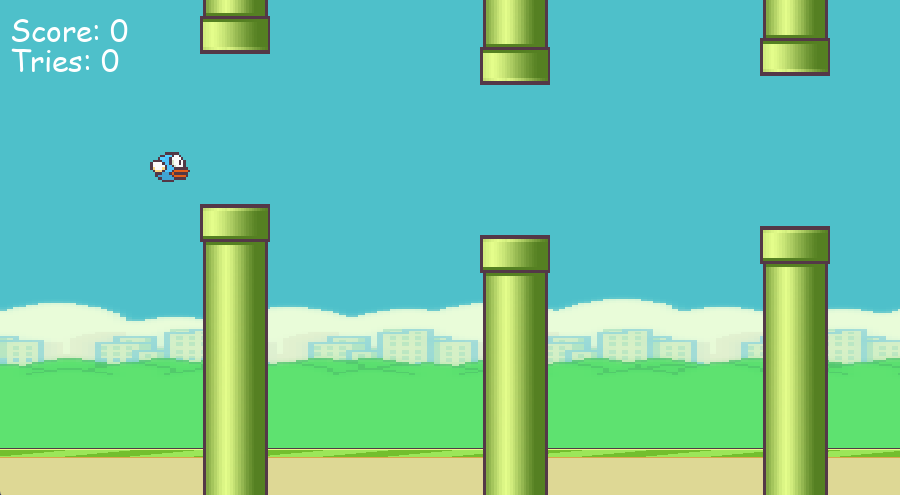
\includegraphics[width=0.9\textwidth, height=0.5\textwidth]{resources/flappy_bird.png}}
%     \centering
%     \caption{Flappy Bird game environment.}
%     \label{fig:problem}
% \end{figure}

\section{METHODS}
The Flappy Bird AI agent in this study is developed using a Deep Q-Learning (DQN) algorithm. The agent learns by interacting with the game environment, making decisions based on the current game state and receiving rewards for actions that avoid losing the game. The agent is given the following information about the state of the game:
\begin{enumerate}
    \item Horizontal distance to next pipe.
    \item Vertical distance to lower next pipe.
    \item Bird's current velocity.
\end{enumerate}
Unlike many implementations of DQN that use Convolutional Neural Networks (CNNs) for feature extraction from images \cite{dutta2018reinforcement}, this agent uses a simple feedforward neural network. The network takes the state vector as input and outputs Q-values corresponding to the two possible actions: flap or do nothing. \\ The agent's learning process is illustrated in Figure \ref{fig:dqn-method}, showing the gathered information from the environment to the agent and the feedback loop for learning.

\begin{figure}[ht!]
    \centering
    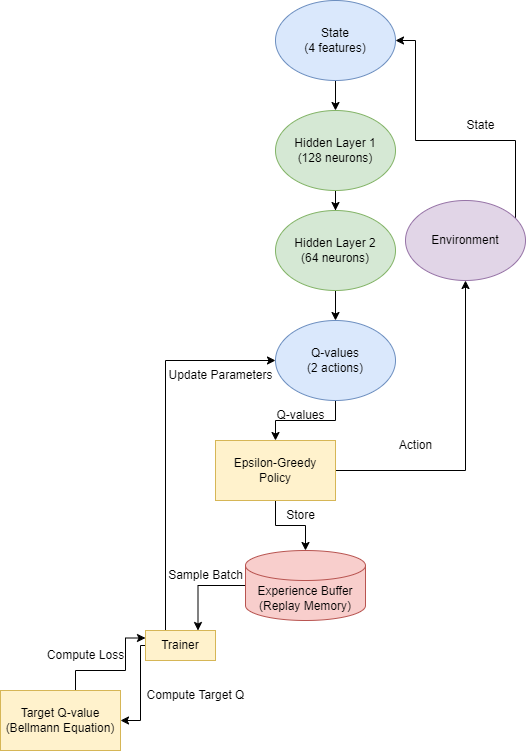
\includegraphics[width=0.5\textwidth, height=0.46\textwidth]{resources/DQN_diagram.png}
    \caption{Method schematic showing the DQN learning process.}
    \label{fig:dqn-method}
\end{figure}

\section{APPLICATIONS}
The agent was trained for up to 250 iterations or until it achieved two consecutive games with scores exceeding 100 points. Due to the simple action space of Flappy Bird, the algorithm converged relatively quickly. During training, the agent balanced exploration and exploitation to optimize its decision-making and achieve high scores.

The hyperparameters used in the training process are summarized in Table \ref{tab:hyperparameters}.

\begin{table}[h!]
\centering
\caption{Training Hyperparameters for the Flappy Bird AI Agent.}
\label{tab:hyperparameters}
\begin{tabular}{|l|c|}
\hline
\textbf{Hyperparameter} & \textbf{Value} \\
\hline
Learning rate \(\alpha\) & 0.001 \\
Discount factor \(\gamma\) & 0.95 \\
Batch size & 128 \\
Replay buffer size & 20,000 \\
Exploration decay \(\epsilon\) & From 1.0 to 0.1 over time \\
\hline
\end{tabular}
\end{table}

With the selected hyperparameters, the agent's performance varies during training. While the algorithm generally converges, it will occasionally diverge which results in suboptimal behaviour as shown in Table \ref{tab:training_results}

% \begin{figure}[h!]
%     \centering
%     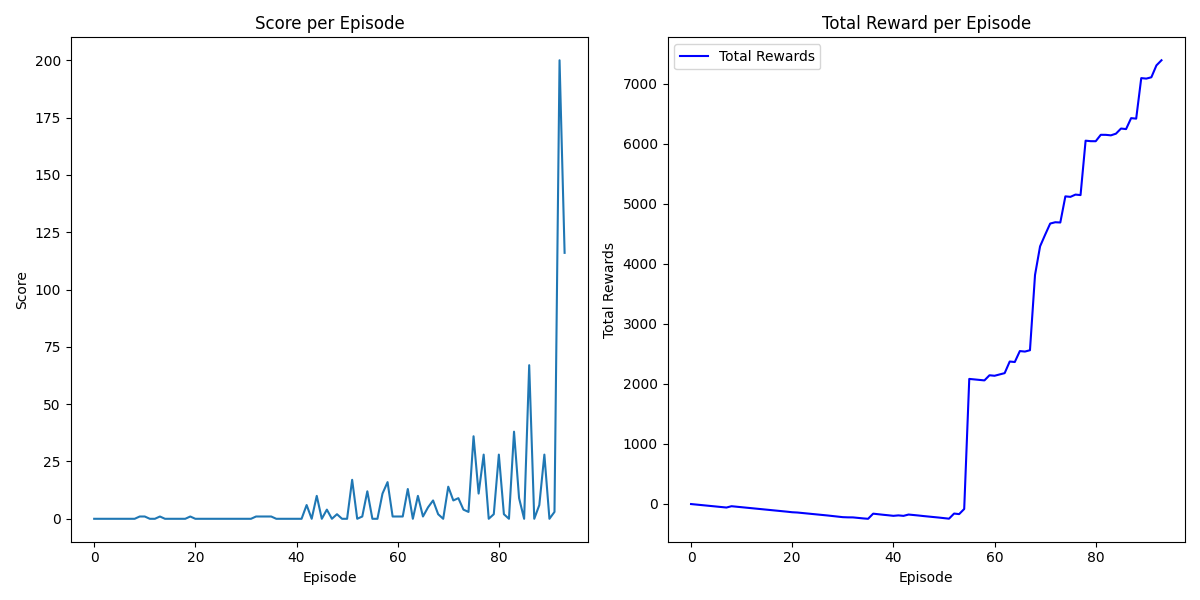
\includegraphics[width=0.9\textwidth, height=0.5\textwidth]{resources/performance_selected.png}
%     \caption{Agent performance: Scores and rewards over training iterations.}
%     \label{fig:nice-graph} 
% \end{figure}

\begin{table}[h!]
    \caption{Training results: Iterations required for the agent to reach 100 points or fail (i.e., 250 iterations).}
    \label{tab:training_results}
    \centering
    \small
    \begin{tabular}{|l|r|}
        \hline
        \textbf{Training Session} & \textbf{Iterations to Reach 100 Points or Fail} \\
        \hline
        1 & 99 \\
        2 & 250 \\
        3 & 250 \\
        4 & 90 \\
        5 & 250 \\
        6 & 250 \\
        7 & 105 \\
        8 & 95 \\
        9 & 94 \\
        10 & 97 \\
        \hline
        Average & 158 \\
        \hline
    \end{tabular}
\end{table}

\newpage
\section{CONCLUSION}
In this case study, the AI agent took an average of 158 iterations to learn how to achieve a score of  100 in Flappy Bird. The agent was able to find an optimal solution about 60\% of the time. While the agent never failed miserably in the other cases, it was unable to reach the score of 100 points before 250 iterations of training.

Overall, these results show that reinforcement learning can work well in this kind of environment, but it’s clear that the agent's performance depends heavily on the chosen hyperparameters. For future work, fine-tuning the algorithm such as by using convolutional neural networks and optimizing the hyperparameters, to enhance the agent's performance and reliability.

% Bibliography
% The name of the BibTeX file is given here. 
% Make sure that your BibTeX file contains all needed bibliographical details. 

\addcontentsline{toc}{section}{REFERENCES}
\bibliography{resources/references}


%% ----------------------- APPENDICES ------------------------------

% \appendix
 
% \section{Taulukot}

% Taulukoita

% \newpage

% \section{Kuvat}

% Kuvia

\end{document}
